\documentclass[tikz,border=14pt]{standalone}
\usepackage[utf8]{inputenc}
\usepackage[T1]{fontenc}
\usepackage{lmodern}
\usepackage{amsmath,amssymb}
\usetikzlibrary{arrows.meta,positioning,calc,fit,backgrounds}

\definecolor{stagebg}{HTML}{DCE4F0}
\definecolor{stageborder}{HTML}{4F627A}
\definecolor{cardbg}{HTML}{FFFFFF}
\definecolor{cardborder}{HTML}{7B8CA3}
\definecolor{probadge}{HTML}{1B4F91}
\definecolor{flashbadge}{HTML}{0D7A5F}
\definecolor{gatebg}{HTML}{E6F4EA}
\definecolor{gateborder}{HTML}{1E8E3E}
\definecolor{revbg}{HTML}{FEF4E2}
\definecolor{revborder}{HTML}{D47A1E}
\definecolor{hitlbg}{HTML}{F3E8FD}
\definecolor{hitlborder}{HTML}{7E3AF2}
\definecolor{finalbg}{HTML}{E6F4EA}
\definecolor{finalborder}{HTML}{237837}
\definecolor{rollbackbg}{HTML}{FCE8E6}
\definecolor{rollbackred}{HTML}{C5221F}
\definecolor{arrowdark}{HTML}{243242}

\begin{document}
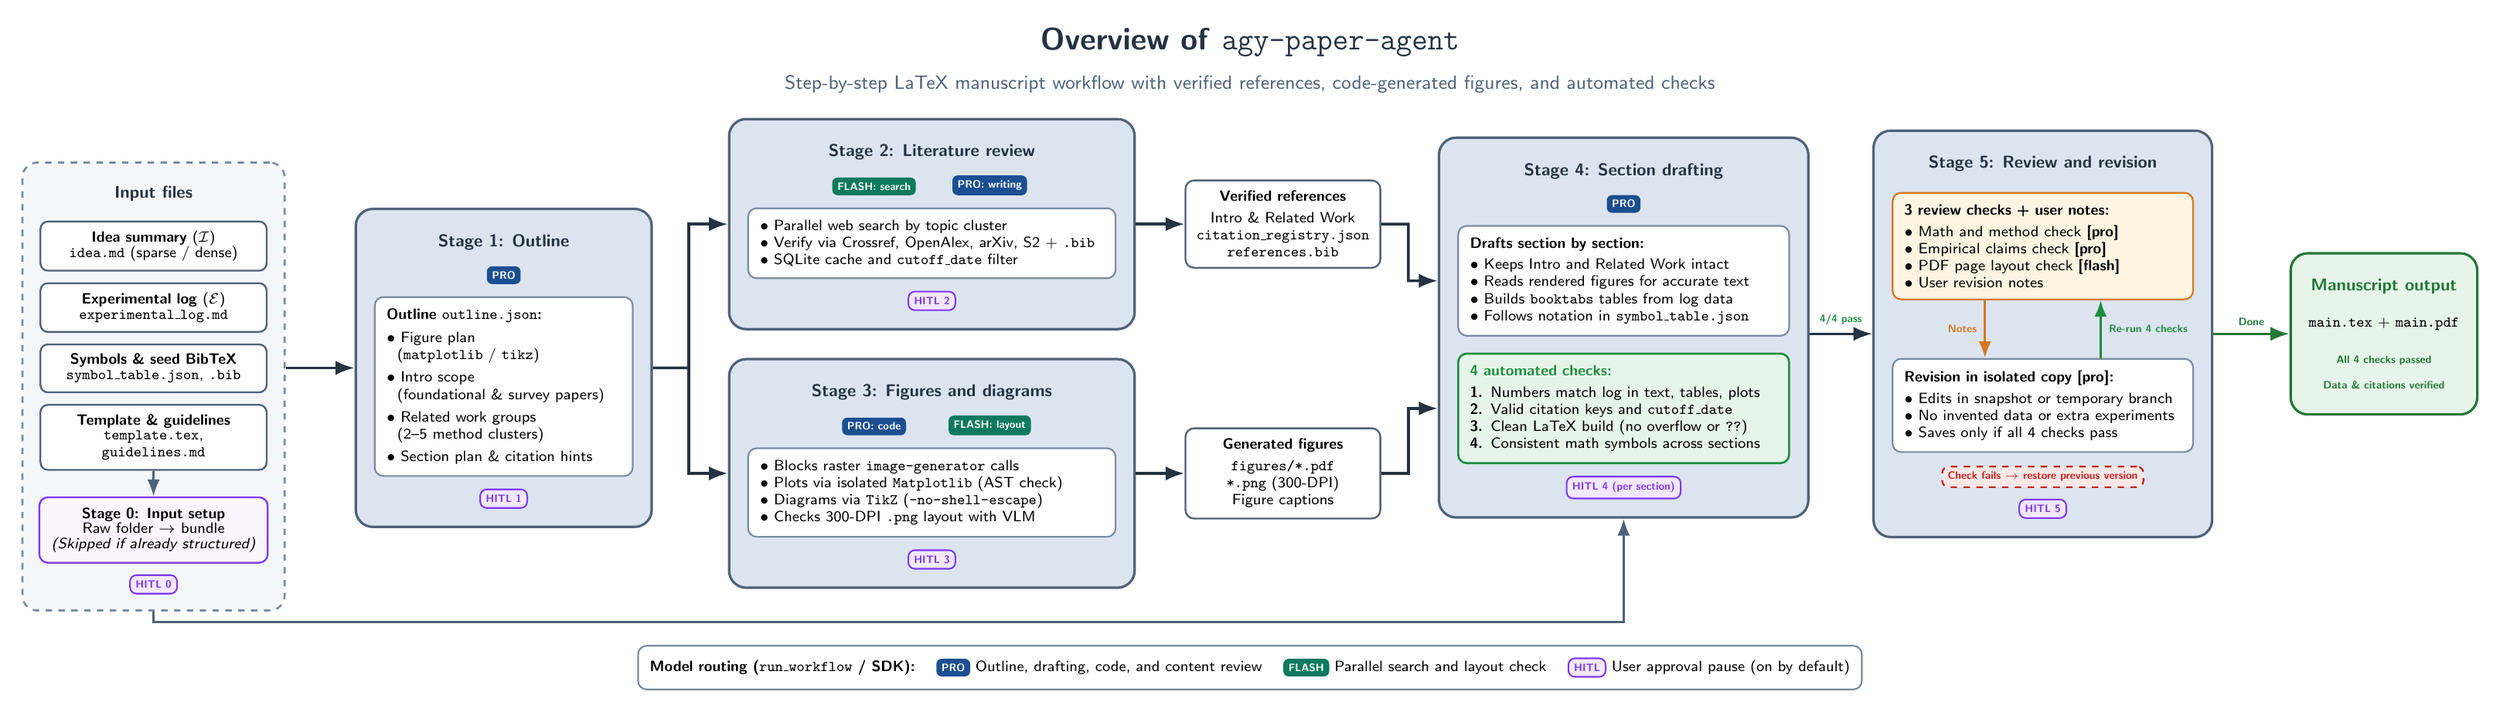
\begin{tikzpicture}[
    font=\sffamily,
    >=Latex,
    stagebox/.style={
        draw=stageborder,
        line width=1.15pt,
        rounded corners=8pt,
        fill=stagebg,
        inner sep=8.5pt
    },
    subcard/.style={
        draw=cardborder,
        line width=0.8pt,
        rounded corners=4pt,
        fill=cardbg,
        align=left,
        font=\sffamily\scriptsize,
        inner sep=5.5pt
    },
    centercard/.style={
        draw=stageborder,
        line width=0.85pt,
        rounded corners=4pt,
        fill=cardbg,
        align=center,
        font=\sffamily\scriptsize,
        inner sep=5pt
    },
    matcard/.style={
        draw=stageborder,
        line width=0.85pt,
        rounded corners=3.5pt,
        fill=cardbg,
        align=center,
        font=\sffamily\scriptsize,
        text width=3.40cm,
        inner sep=4.5pt
    },
    gatecard/.style={
        draw=gateborder,
        line width=0.95pt,
        rounded corners=4pt,
        fill=gatebg,
        align=left,
        font=\sffamily\scriptsize,
        inner sep=5.5pt
    },
    hitlpill/.style={
        draw=hitlborder,
        line width=0.75pt,
        rounded corners=3pt,
        fill=hitlbg,
        text=hitlborder,
        font=\sffamily\bfseries\tiny,
        inner sep=2.6pt
    },
    rollbackpill/.style={
        draw=rollbackred,
        dashed,
        line width=0.8pt,
        rounded corners=3pt,
        fill=rollbackbg,
        text=rollbackred,
        font=\sffamily\bfseries\tiny,
        inner sep=2.6pt
    },
    protag/.style={
        fill=probadge,
        text=white,
        rounded corners=2.5pt,
        font=\sffamily\bfseries\tiny,
        inner sep=2.4pt
    },
    flashtag/.style={
        fill=flashbadge,
        text=white,
        rounded corners=2.5pt,
        font=\sffamily\bfseries\tiny,
        inner sep=2.4pt
    },
    flowarrow/.style={->, line width=1.3pt, draw=arrowdark},
    busarrow/.style={->, line width=1.1pt, draw=stageborder}
]

% ================= COL 0: INPUT FILES & STAGE 0 =================
\node[font=\sffamily\bfseries\footnotesize, text=arrowdark] (in_hdr) at (0, 0) {Input files};
\node[matcard, below=5.5pt of in_hdr] (in_idea) {\textbf{Idea summary} ($\mathcal{I}$)\\[-1pt]\texttt{idea.md} (sparse / dense)};
\node[matcard, below=5pt of in_idea]  (in_log)  {\textbf{Experimental log} ($\mathcal{E}$)\\[-1pt]\texttt{experimental\_log.md}};
\node[matcard, below=5pt of in_log]   (in_sym)  {\textbf{Symbols \& seed BibTeX}\\[-1pt]\texttt{symbol\_table.json}, \texttt{.bib}};
\node[matcard, below=5pt of in_sym]   (in_tpl)  {\textbf{Template \& guidelines}\\[-1pt]\texttt{template.tex}, \texttt{guidelines.md}};

\node[centercard, fill=hitlbg!45, draw=hitlborder, text width=3.40cm, below=12pt of in_tpl] (st0)
    {\textbf{Stage 0: Input setup}\\[-1pt]Raw folder $\to$ bundle\\[-1pt]\textit{(Skipped if already structured)}};
\node[hitlpill, below=5pt of st0] (hitl0) {HITL 0};

\begin{scope}[on background layer]
    \node[draw=cardborder, dashed, line width=0.95pt, rounded corners=7pt, fill=stagebg!30,
          fit=(in_hdr)(in_idea)(in_tpl)(st0)(hitl0), inner sep=7.5pt] (input_group) {};
\end{scope}

% ================= COL 1: STAGE 1 OUTLINE =================
\node[subcard, text width=3.85cm, right=1.45cm of input_group] (st1_card) {
    \textbf{Outline \texttt{outline.json}:}\\[3pt]
    $\bullet$ Figure plan\\
    \hspace{5pt}(\texttt{matplotlib} / \texttt{tikz})\\[2.5pt]
    $\bullet$ Intro scope\\
    \hspace{5pt}(foundational \& survey papers)\\[2.5pt]
    $\bullet$ Related work groups\\
    \hspace{5pt}(2--5 method clusters)\\[2.5pt]
    $\bullet$ Section plan \& citation hints
};
\node[protag, above=5.5pt of st1_card] (st1_tag) {PRO};
\node[font=\sffamily\bfseries\footnotesize, text=arrowdark, above=4pt of st1_tag] (st1_hdr) {Stage 1: Outline};
\node[hitlpill, below=5.5pt of st1_card] (hitl1) {HITL 1};

\begin{scope}[on background layer]
    \node[stagebox, fit=(st1_hdr)(st1_tag)(st1_card)(hitl1)] (st1_box) {};
\end{scope}

% ================= COL 2 TOP: STAGE 2 LITERATURE =================
\node[subcard, text width=5.65cm, anchor=west] (st2_card) at ([xshift=1.55cm, yshift=2.05cm]st1_box.east) {
    $\bullet$ Parallel web search by topic cluster\\
    $\bullet$ Verify via Crossref, OpenAlex, arXiv, S2 + \texttt{.bib}\\
    $\bullet$ SQLite cache and \texttt{cutoff\_date} filter
};
\node[flashtag, above=5.5pt of st2_card.north, xshift=-0.95cm] (st2_t1) {FLASH: search};
\node[protag,   above=5.5pt of st2_card.north, xshift=0.95cm]  (st2_t2) {PRO: writing};
\coordinate (st2_tmid) at ($(st2_t1.north)!0.5!(st2_t2.north)$);
\node[font=\sffamily\bfseries\footnotesize, text=arrowdark, above=4pt of st2_tmid] (st2_hdr) {Stage 2: Literature review};
\node[hitlpill, below=5.5pt of st2_card] (hitl2) {HITL 2};

\begin{scope}[on background layer]
    \node[stagebox, fit=(st2_hdr)(st2_t1)(st2_t2)(st2_card)(hitl2)] (st2_box) {};
\end{scope}

% ================= COL 2 BOTTOM: STAGE 3 FIGURES =================
\node[subcard, text width=5.65cm, anchor=west] (st3_card) at ([xshift=1.55cm, yshift=-2.05cm]st1_box.east) {
    $\bullet$ Blocks raster \texttt{image-generator} calls\\
    $\bullet$ Plots via isolated \texttt{Matplotlib} (AST check)\\
    $\bullet$ Diagrams via \texttt{TikZ} (\texttt{-no-shell-escape})\\
    $\bullet$ Checks 300-DPI \texttt{.png} layout with VLM
};
\node[protag,   above=5.5pt of st3_card.north, xshift=-0.95cm] (st3_t1) {PRO: code};
\node[flashtag, above=5.5pt of st3_card.north, xshift=0.95cm]  (st3_t2) {FLASH: layout};
\coordinate (st3_tmid) at ($(st3_t1.north)!0.5!(st3_t2.north)$);
\node[font=\sffamily\bfseries\footnotesize, text=arrowdark, above=4pt of st3_tmid] (st3_hdr) {Stage 3: Figures and diagrams};
\node[hitlpill, below=5.5pt of st3_card] (hitl3) {HITL 3};

\begin{scope}[on background layer]
    \node[stagebox, fit=(st3_hdr)(st3_t1)(st3_t2)(st3_card)(hitl3)] (st3_box) {};
\end{scope}

% Mid-output cards
\node[centercard, text width=2.85cm, right=0.80cm of st2_box] (out_lit) {
    \textbf{Verified references}\\[2pt]
    Intro \& Related Work\\
    \texttt{citation\_registry.json}\\
    \texttt{references.bib}
};
\node[centercard, text width=2.85cm, right=0.80cm of st3_box] (out_figs) {
    \textbf{Generated figures}\\[2pt]
    \texttt{figures/*.pdf}\\
    \texttt{*.png} (300-DPI)\\
    Figure captions
};

% ================= COL 3: STAGE 4 SECTION DRAFTING + 4 CHECKS =================
\coordinate (mid_col2) at ($(out_lit.east)!0.5!(out_figs.east)$);
\node[subcard, text width=5.05cm, anchor=south west] (st4_draft) at ([xshift=1.25cm, yshift=0.20cm]mid_col2) {
    \textbf{Drafts section by section:}\\[2pt]
    $\bullet$ Keeps Intro and Related Work intact\\
    $\bullet$ Reads rendered figures for accurate text\\
    $\bullet$ Builds \texttt{booktabs} tables from log data\\
    $\bullet$ Follows notation in \texttt{symbol\_table.json}
};
\node[protag, above=5.5pt of st4_draft] (st4_tag) {PRO};
\node[font=\sffamily\bfseries\footnotesize, text=arrowdark, above=4pt of st4_tag] (st4_hdr) {Stage 4: Section drafting};

\node[gatecard, text width=5.05cm, below=7.5pt of st4_draft] (st4_gates) {
    \textbf{\textcolor{gateborder}{4 automated checks:}}\\[2pt]
    \textbf{1.} Numbers match log in text, tables, plots\\
    \textbf{2.} Valid citation keys and \texttt{cutoff\_date}\\
    \textbf{3.} Clean LaTeX build (no overflow or \texttt{??})\\
    \textbf{4.} Consistent math symbols across sections
};
\node[hitlpill, below=5.5pt of st4_gates] (hitl4) {HITL 4 (per section)};

\begin{scope}[on background layer]
    \node[stagebox, fit=(st4_hdr)(st4_tag)(st4_draft)(st4_gates)(hitl4)] (st4_box) {};
\end{scope}

% ================= COL 4: STAGE 5 REVIEW AND REVISION =================
\node[subcard, fill=revbg, draw=revborder, text width=4.55cm, anchor=south west] (st5_panel) at ([xshift=1.35cm, yshift=0.45cm]st4_box.east) {
    \textbf{3 review checks + user notes:}\\[2pt]
    $\bullet$ Math and method check \textbf{[pro]}\\
    $\bullet$ Empirical claims check \textbf{[pro]}\\
    $\bullet$ PDF page layout check \textbf{[flash]}\\
    $\bullet$ User revision notes
};
\node[font=\sffamily\bfseries\footnotesize, text=arrowdark, above=6pt of st5_panel] (st5_hdr) {Stage 5: Review and revision};

\node[subcard, text width=4.55cm, below=0.95cm of st5_panel] (st5_rev) {
    \textbf{Revision in isolated copy [pro]:}\\[2pt]
    $\bullet$ Edits in snapshot or temporary branch\\
    $\bullet$ No invented data or extra experiments\\
    $\bullet$ Saves only if all 4 checks pass
};
\node[rollbackpill, below=6pt of st5_rev] (st5_rb) {Check fails $\to$ restore previous version};
\node[hitlpill, below=5pt of st5_rb]      (hitl5)  {HITL 5};

\begin{scope}[on background layer]
    \node[stagebox, fit=(st5_hdr)(st5_panel)(st5_rev)(st5_rb)(hitl5)] (st5_box) {};
\end{scope}

% Internal loop arrows inside Stage 5
\draw[->, line width=1.05pt, draw=revborder]
    ([xshift=-0.95cm]st5_panel.south) -- node[left, font=\sffamily\bfseries\tiny, text=revborder] {Notes}
    ([xshift=-0.95cm]st5_rev.north);
\draw[->, line width=1.05pt, draw=gateborder]
    ([xshift=0.95cm]st5_rev.north) -- node[right, font=\sffamily\bfseries\tiny, text=gateborder] {Re-run 4 checks}
    ([xshift=0.95cm]st5_panel.south);

% ================= COL 5: FINAL OUTPUT =================
\node[stagebox, fill=finalbg, draw=finalborder, align=center, minimum width=3.05cm, minimum height=2.65cm, right=1.25cm of st5_box] (final_box) {
    \textbf{\textcolor{finalborder}{\footnotesize Manuscript output}}\\[5pt]
    \scriptsize\texttt{main.tex} + \texttt{main.pdf}\\[5pt]
    \tiny\textbf{\textcolor{finalborder}{All 4 checks passed}}\\
    \tiny\textbf{\textcolor{finalborder}{Data \& citations verified}}
};

% ================= CONNECTIONS =================
\draw[busarrow] (in_tpl.south) -- (st0.north);
\draw[flowarrow] (input_group.east |- st1_box.west) -- (st1_box.west);

% Split from Stage 1 to Stage 2 (top) and Stage 3 (bottom)
\coordinate (split_pt) at ($(st1_box.east)!0.48!(st2_box.west |- st1_box.east)$);
\draw[line width=1.3pt, draw=arrowdark] (st1_box.east) -- (split_pt);
\draw[flowarrow] (split_pt) |- (st2_box.west);
\draw[flowarrow] (split_pt) |- (st3_box.west);

% Stage 2 & Stage 3 to intermediate outputs and into Stage 4
\draw[flowarrow] (st2_box.east) -- (out_lit.west);
\draw[flowarrow] (st3_box.east) -- (out_figs.west);

\coordinate (merge_x) at ($(out_lit.east)!0.48!(st4_box.west |- out_lit.east)$);
\draw[flowarrow] (out_lit.east)  -- (merge_x) |- (st4_draft.west -| st4_box.west);
\draw[flowarrow] (out_figs.east) -- (merge_x |- out_figs.east) |- (st4_gates.west -| st4_box.west);

% Bottom direct context bus (Input files -> Stage 4)
\coordinate (bus_bottom_y) at ([yshift=-0.55cm]st3_box.south);
\draw[busarrow] (input_group.south) |- (bus_bottom_y -| st4_box.south) -- (st4_box.south);

% Stage 4 -> Stage 5 -> Final Output
\draw[flowarrow] (st4_box.east |- final_box.west) -- node[above, font=\sffamily\bfseries\tiny, text=gateborder] {4/4 pass} (st5_box.west |- final_box.west);
\draw[flowarrow, draw=finalborder] (st5_box.east |- final_box.west) -- node[above, font=\sffamily\bfseries\tiny, text=finalborder] {Done} (final_box.west);

% ================= TITLE BANNER & LEGEND FOOTER =================
\coordinate (diagram_center) at ($(input_group.west)!0.5!(final_box.east)$);
\coordinate (top_anchor) at (current bounding box.north);
\coordinate (bot_anchor) at (current bounding box.south);

\node[font=\sffamily\small, text=stageborder, anchor=south] (sub_title) at (diagram_center |- top_anchor) [yshift=8pt]
    {Step-by-step LaTeX manuscript workflow with verified references, code-generated figures, and automated checks};
\node[font=\sffamily\bfseries\Large, text=arrowdark, above=2pt of sub_title]
    {Overview of \texttt{agy-paper-agent}};

\node[draw=cardborder, line width=0.8pt, rounded corners=4pt, fill=white, inner sep=5.5pt, font=\sffamily\scriptsize, anchor=north] at (diagram_center |- bot_anchor) [yshift=-10pt] {
    \textbf{Model routing (\texttt{run\_workflow} / SDK):} \quad
    \tikz[baseline=(b.base)]\node[protag](b){PRO}; Outline, drafting, code, and content review \quad
    \tikz[baseline=(b.base)]\node[flashtag](b){FLASH}; Parallel search and layout check \quad
    \tikz[baseline=(b.base)]\node[hitlpill](b){HITL}; User approval pause (on by default)
};

\end{tikzpicture}
\end{document}
